\clearpage
\subsubsection{Fluvial}
\begin{table}[h!]
\centering
\caption{Categorised GPR profile keywords for fluvial environments. Geometry, reflectivity and continuity are shown in separate columns.}
\begin{tabular}{|p{5cm}|p{5cm}|p{5cm}|}
\hline
\textbf{Geometry / Structure} & \textbf{Continuity} & \textbf{Amplitude / Reflectivity} \\
\hline
Dipping & Continuous & Low amplitude \\
Horizontal & Semi-continuous & High amplitude \\
Planar & Discontinuous & Medium amplitude \\
Parallel & & Varied reflectivity \\
Concave & & High reflectivity \\
Undulated & & Medium reflectivity \\
Onlap & & low amplitude \\
Toplap & & varied amplitude \\
Sub-horizontal & & continuous \\
Truncation & & \\
Prograding & & \\
Accretionary & & \\
Mounded & & \\
Oblique & & \\
Sigmoidal & & \\
Erosion & & \\
Truncating & & \\
Lenticular & & \\
Multidirectional dipping & & \\
Convex & & \\
Subparallel & & \\
Chaotic & & \\
Cross-bedding & & \\
Faulting & & \\
Crossing reflectors & & \\
Stratification & & \\
\hline
\end{tabular}
\label{tab:fluvial-keywords}
\end{table}

\begin{figure}[h!]
    \centering
    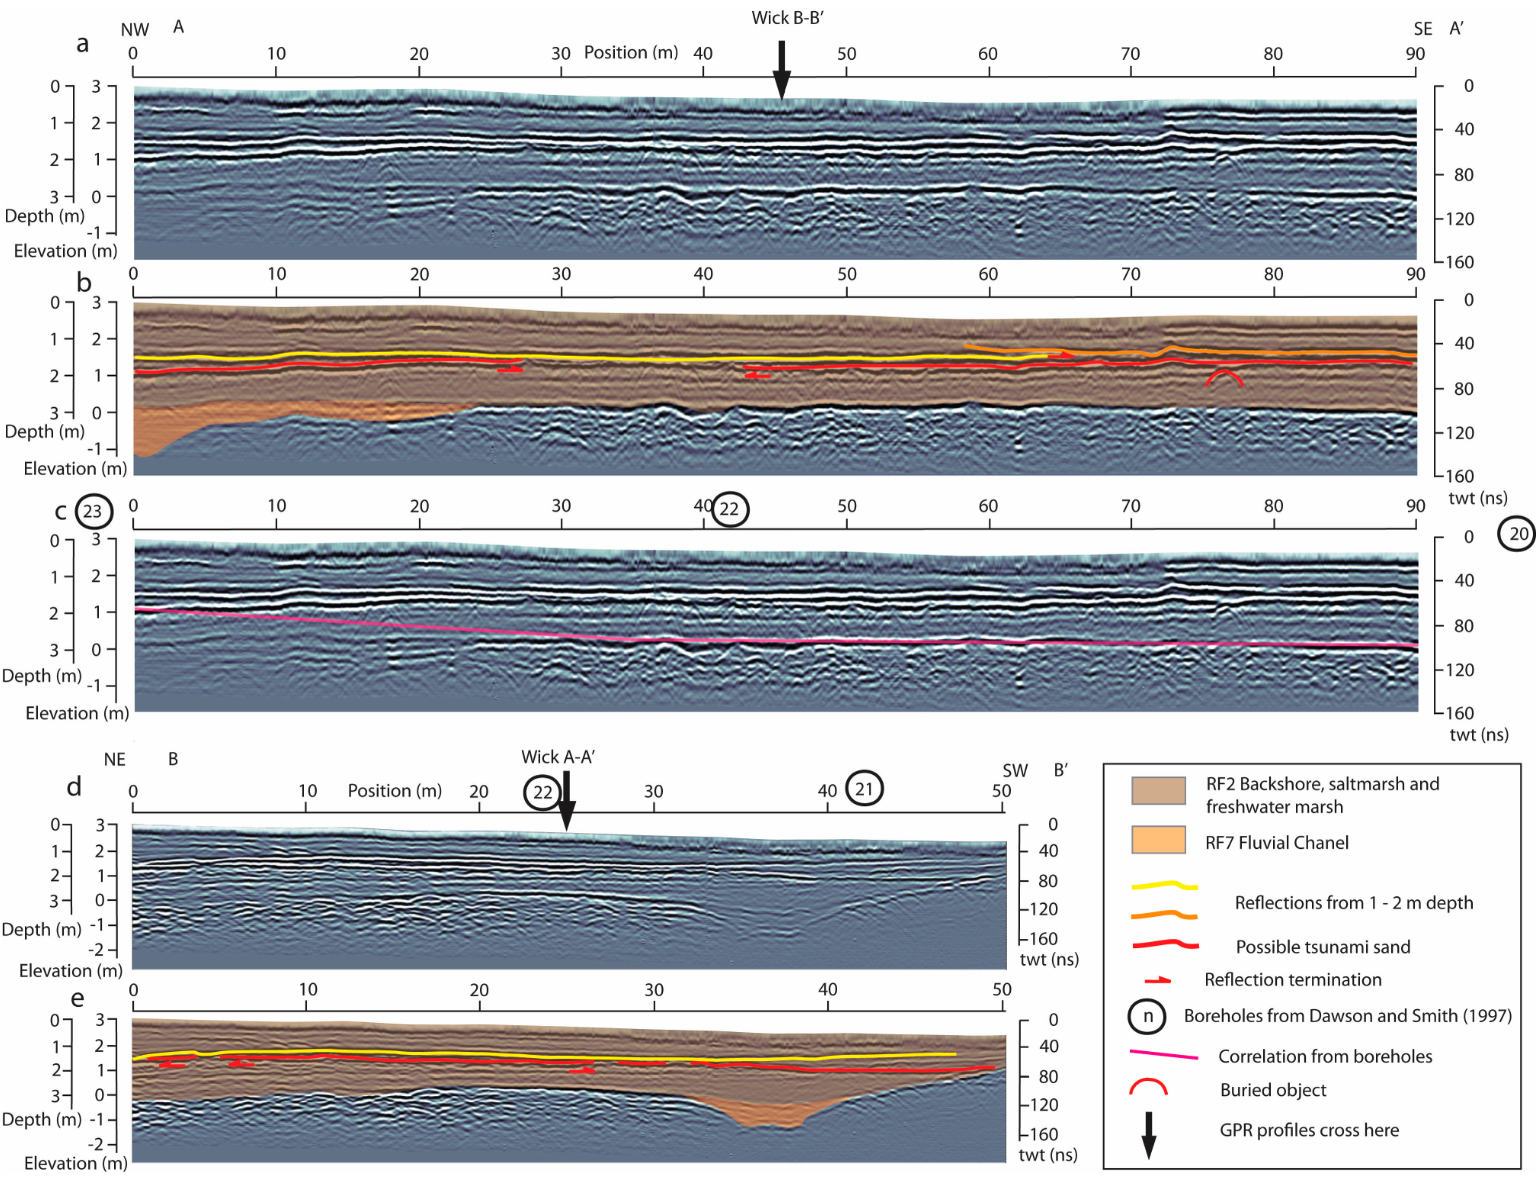
\includegraphics[width=0.9\linewidth]{Figures/0.2GPR/Bristow_2024_1.png}
    \caption[Tsunami sand.]{Tsunami sand.\textbf{Keywords: } Discontinuous, truncation, subparallel \citep{Bristow2024}.}
    \label{fig:Bristow2024-1}
\end{figure}

\begin{figure}[h!]
    \centering
    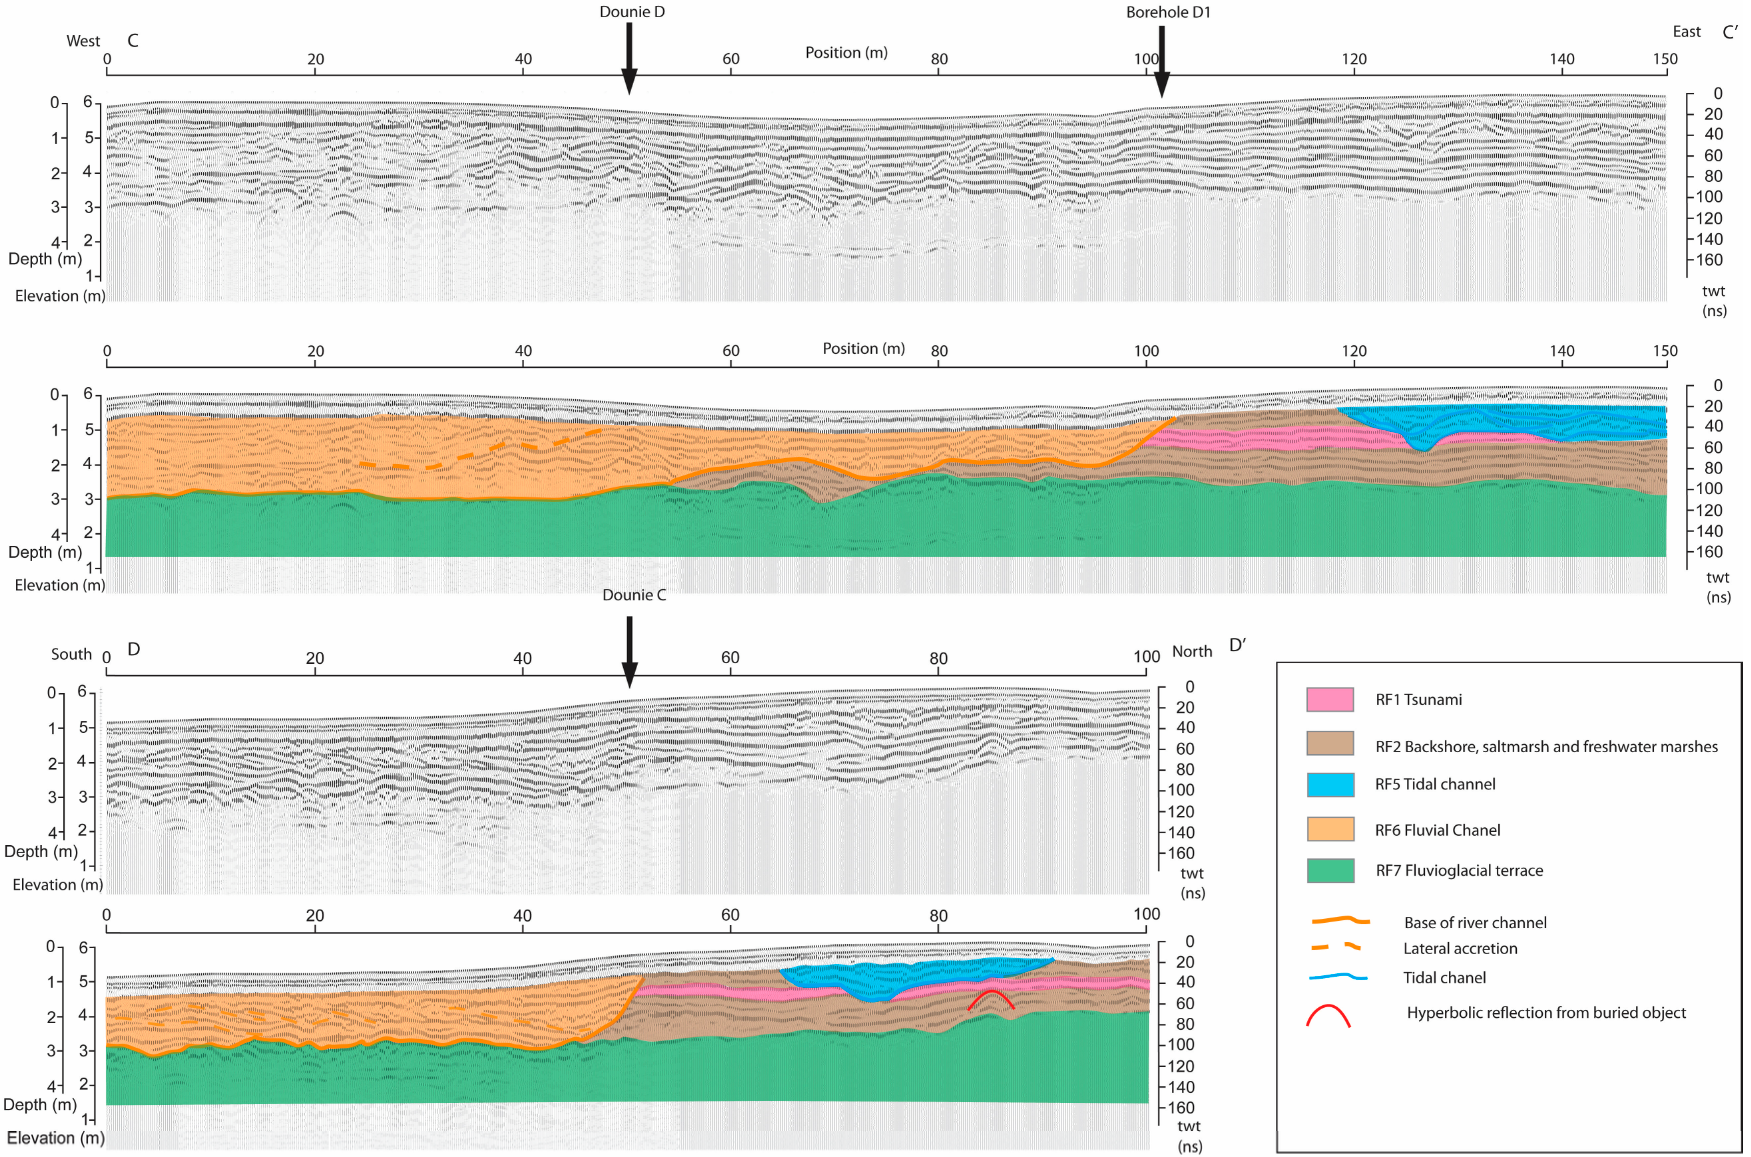
\includegraphics[width=0.9\linewidth]{Figures/0.2GPR/Bristow_2024_5.png}
    \caption[River deposits cutting into tsunami and tidal flat sediments.]{River deposits cutting into tsunami and tidal flat sediments. \textbf{Keywords: } Low amplitude, continuous, varying amplitude, high amplitude, truncating, concave, discontinuous, sub-horizontal, dipping  \citep{Bristow2024}.}
    \label{fig:Bristow2024-5}
\end{figure}

\begin{figure}[h!]
    \centering
    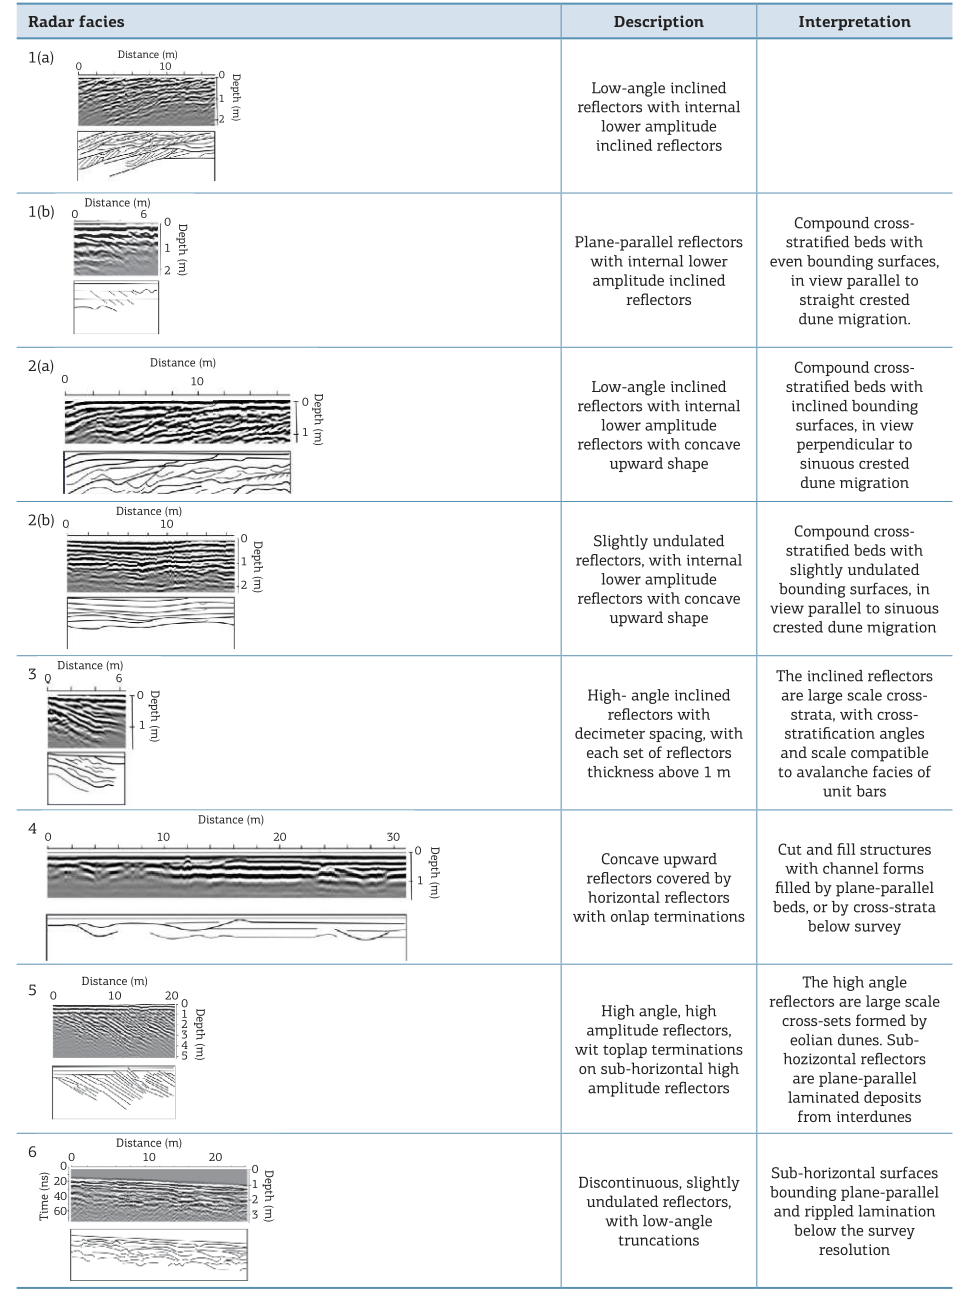
\includegraphics[width=0.9\linewidth]{Figures/0.2GPR/Tamura2016_Fluvial.png}
    \caption[Architectural elements in sedimentary structures.]{Architectural elements in sedimentary structures. \textbf{Keywords: } Dipping, inclined, low amplitude, planar, parallel, concave, undulated, high-angle, horizontal, onlap, high amplitude, toplap, sub-horizontal, discontinuous, truncation \citep{Tamura2016}.}
    \label{fig:Tamura2016-1}
\end{figure}

\begin{figure}[h!]
    \centering
    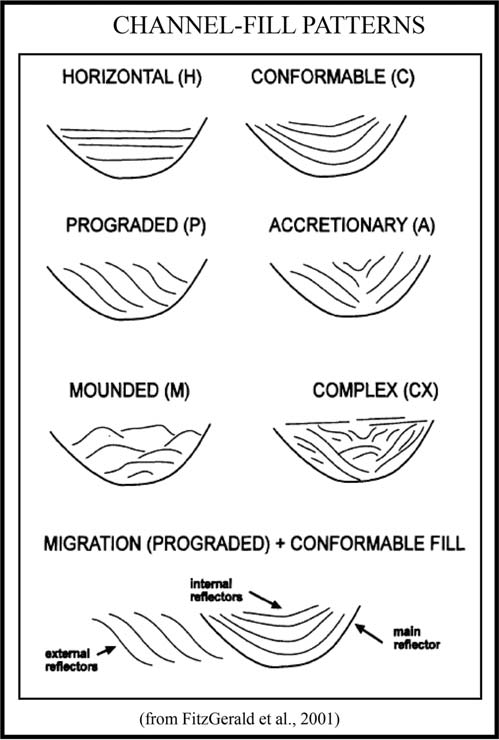
\includegraphics[width=0.9\linewidth]{Figures/0.2GPR/Maio2015_channelfill.png}
    \caption[Storm-Driven Breaching along a Transgressing Barrier System (1).]{Storm-Driven Breaching along a Transgressing Barrier System (1). \textbf{Keywords: } Horizontal, prograding, accretionary, mounded, continuous, semi-continuous, varied reflectivity, onlap, truncating   \citep{Maio2016}.}
    \label{fig:Maio2016-1}
\end{figure}

\begin{figure}[h!]
    \centering
    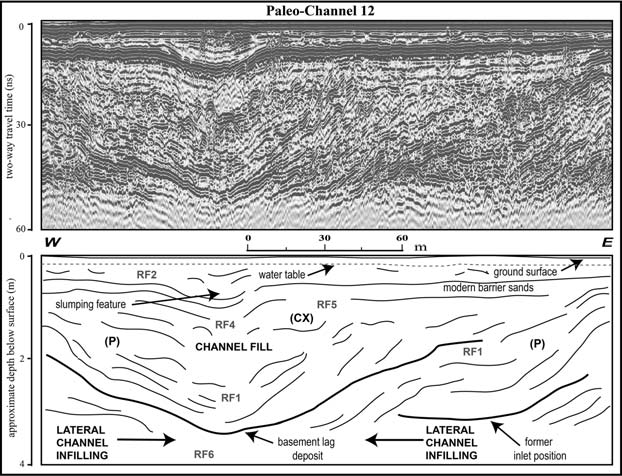
\includegraphics[width=0.9\linewidth]{Figures/0.2GPR/Maio2015_channelfill_2.png}
    \caption[Storm-Driven Breaching along a Transgressing Barrier System (2).]{Storm-Driven Breaching along a Transgressing Barrier System (2).\textbf{Keywords: } Concave, oblique, sigmoidal, discontinuous, semi-continuous, chaotic, varied amplitude, high reflectivity, truncation, erosion, onlap \citep{Maio2016}.}
    \label{fig:Maio2016-2}
\end{figure}


\begin{figure}[h!]
    \centering
    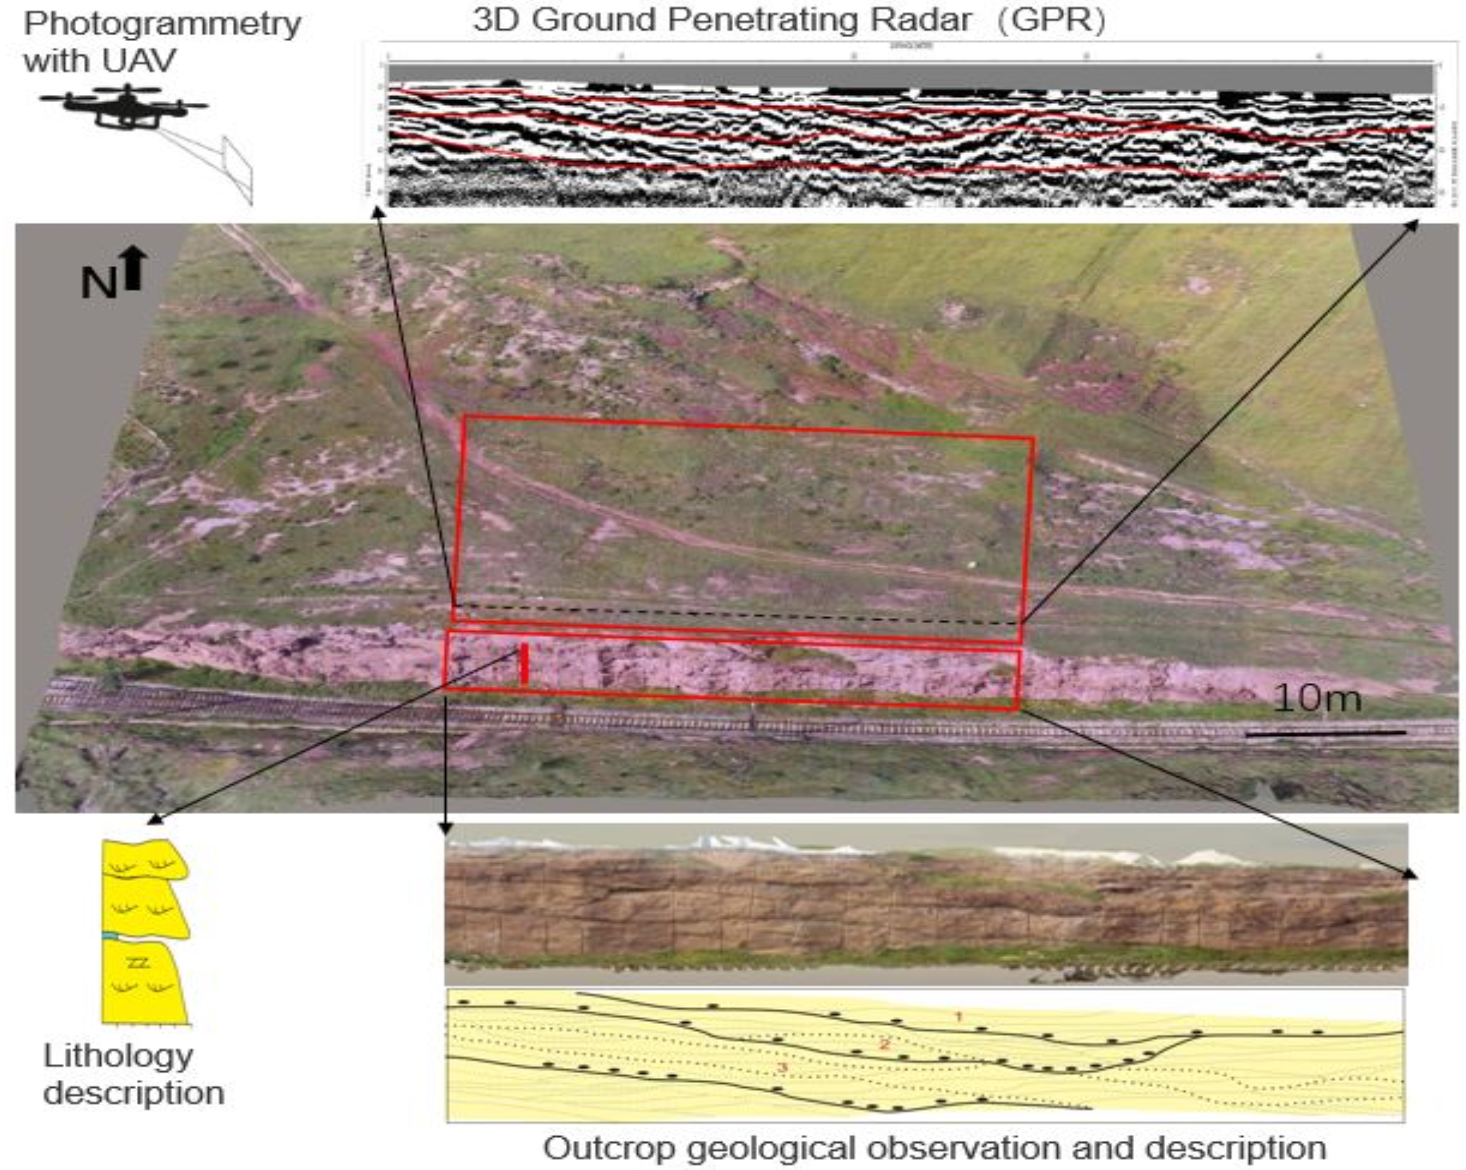
\includegraphics[width=0.9\linewidth]{Figures/0.2GPR/Guo2022_1.png}
    \caption[Sandy Braided River (1).]{Sandy Braided River (1). \textbf{Keywords: } Dipping, continuous, semi-continuous, parallel, concave, lenticular, high reflectivity \citep{Guo2022}.}
    \label{fig:Guo2022-1}
\end{figure}


\begin{figure}[h!]
    \centering
    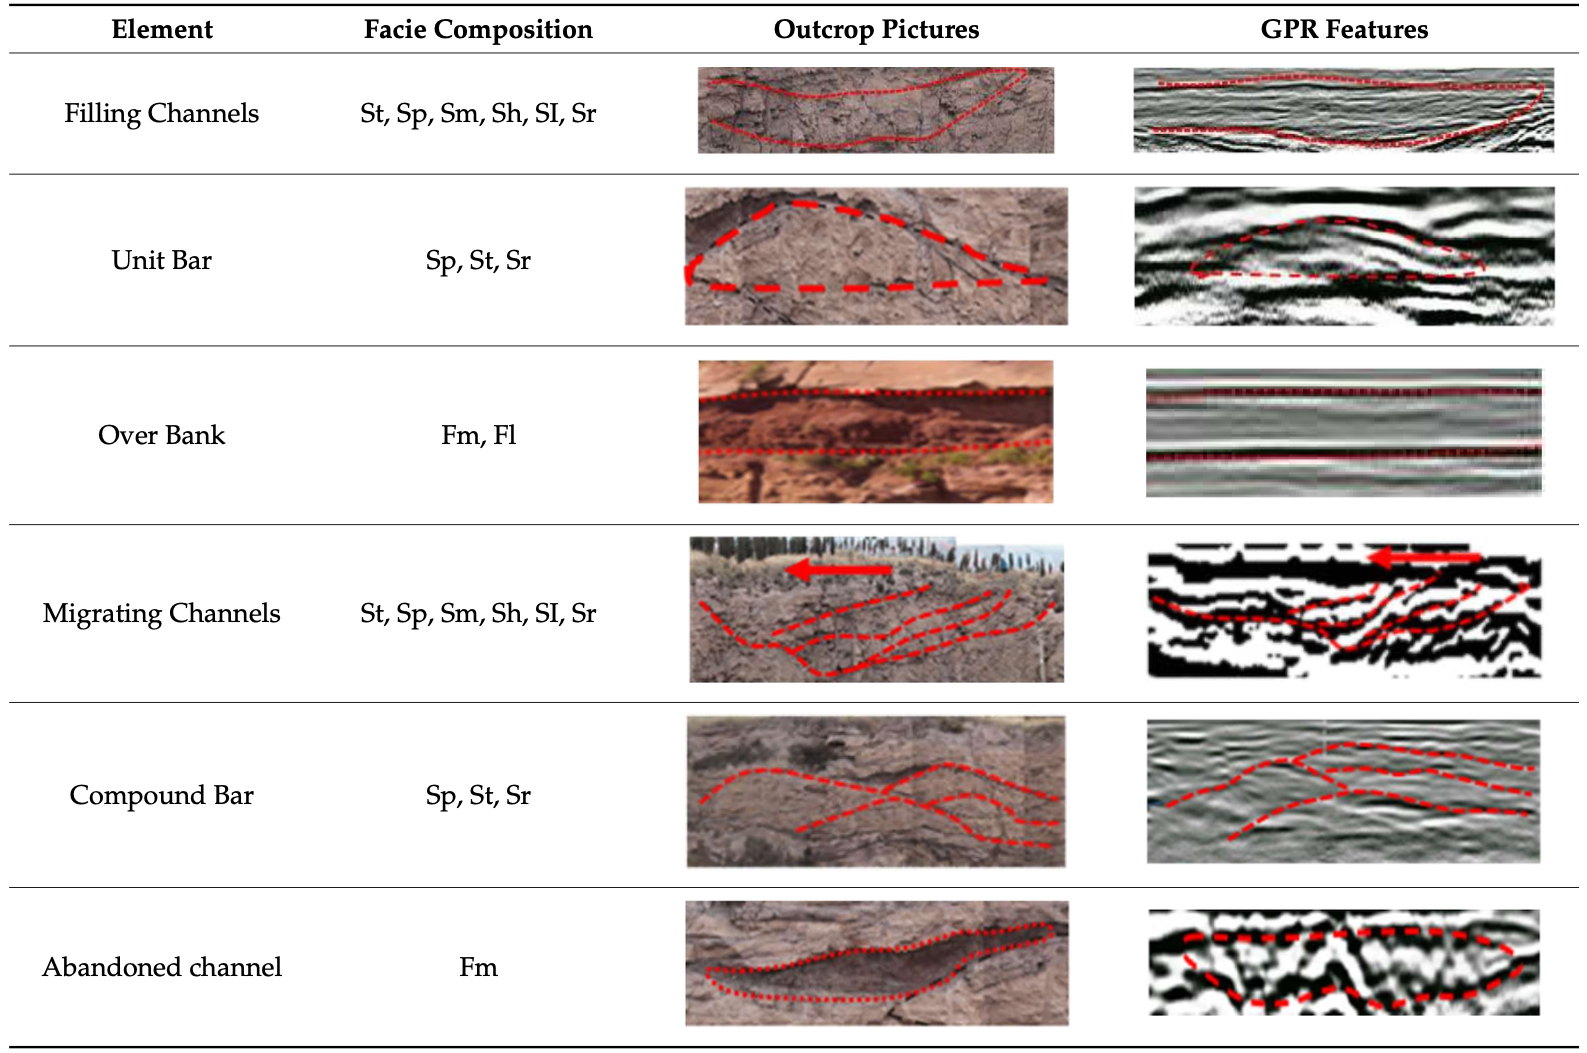
\includegraphics[width=0.9\linewidth]{Figures/0.2GPR/Guo2022_6.png}
    \caption[Sandy Braided River (2).]{Sandy Braided River (2). \textbf{Keywords: } Lenticular, multidirectional dipping, onlap, semi-horizontal, hummocky, concave, varied reflectivity, continuous, discontinuous \citep{Guo2022}.}
    \label{fig:Guo2022-6}
\end{figure}

\begin{figure}[h!]
    \centering
    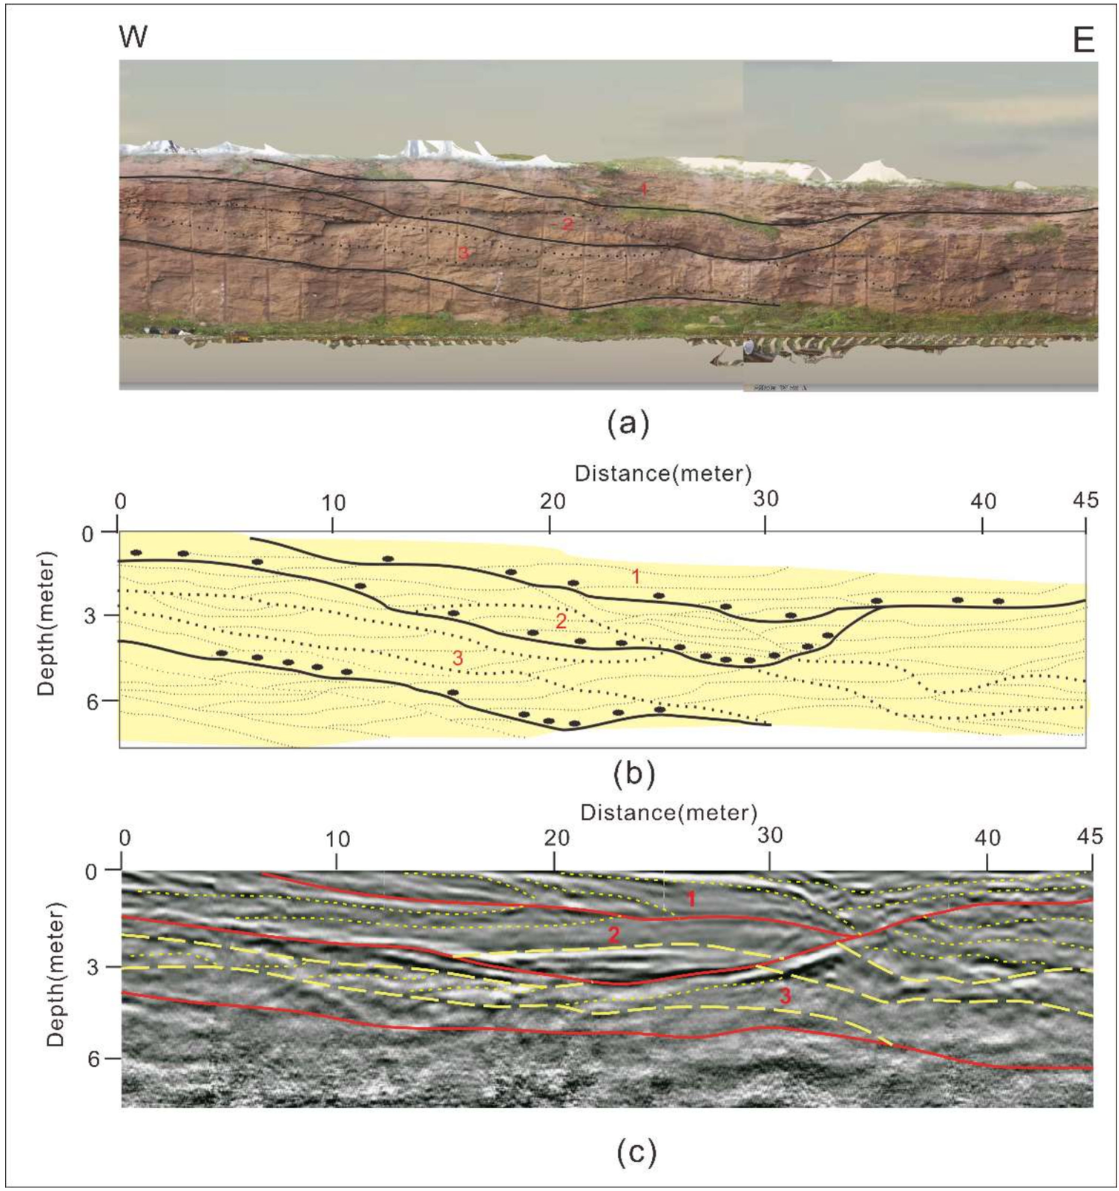
\includegraphics[width=0.9\linewidth]{Figures/0.2GPR/Guo2022_5.png}
    \caption[Sandy Braided River (3).]{Sandy Braided River (3). \textbf{Keywords:} Lenticular, horizontal, convex-down, parallel, subparallel, chaotic, low amplitude \citep{Guo2022}.}
    \label{fig:Guo2022-5}
\end{figure}


\begin{figure}[h!]
    \centering
    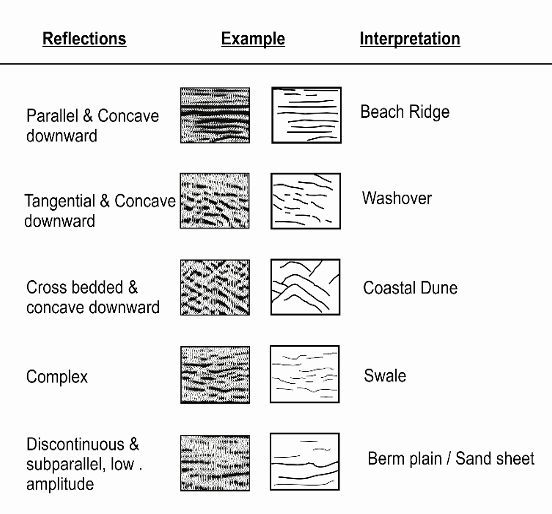
\includegraphics[width=0.9\linewidth]{Figures/0.2GPR/Shukla2013_Coastal_margin.png}
    \caption[Sedimentary architecture and coastal dynamics.]{Sedimentary architecture and coastal dynamics. \textbf{Keywords: } Parallel, concave, cross-bedding, discontinuous, subparallel, low amplitude, horizontal, dipping \citep{Shukla2013}.}
    \label{fig:Shukla2013-1}
\end{figure}

\begin{figure}[h!]
    \centering
    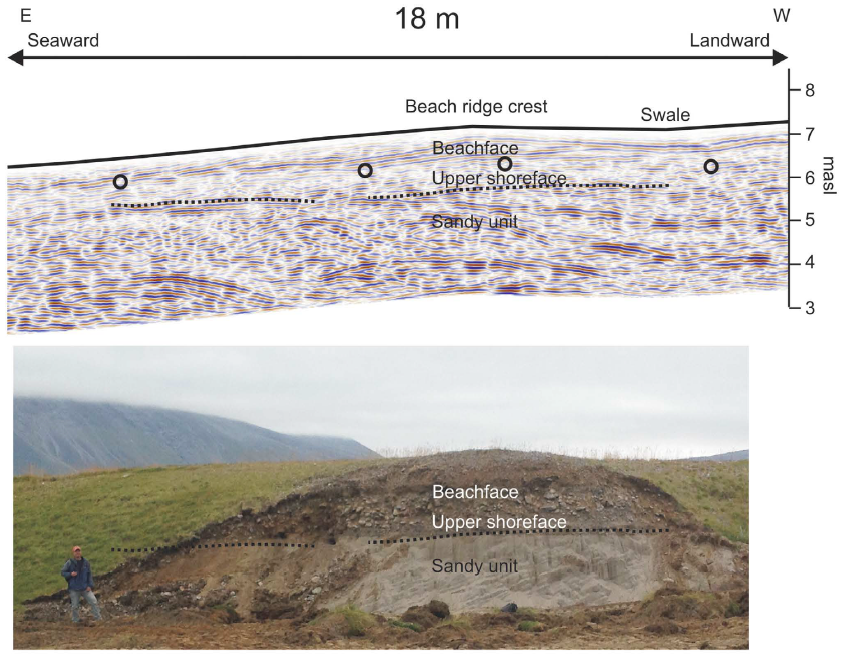
\includegraphics[width=0.9\linewidth]{Figures/0.2GPR/Nielsen_2017_beach.png}
    \caption[Beach ridge eroded by river.]{Beach ridge eroded by river. \textbf{Keywords: } Dipping, medium reflectivity, semi-continuous, hummocky, truncation, erosion, semi-horizontal \citep{Nielsen2017}.}
    \label{fig:Nielsen2017-beach-1}
\end{figure}

\begin{figure}[h!]
    \centering
    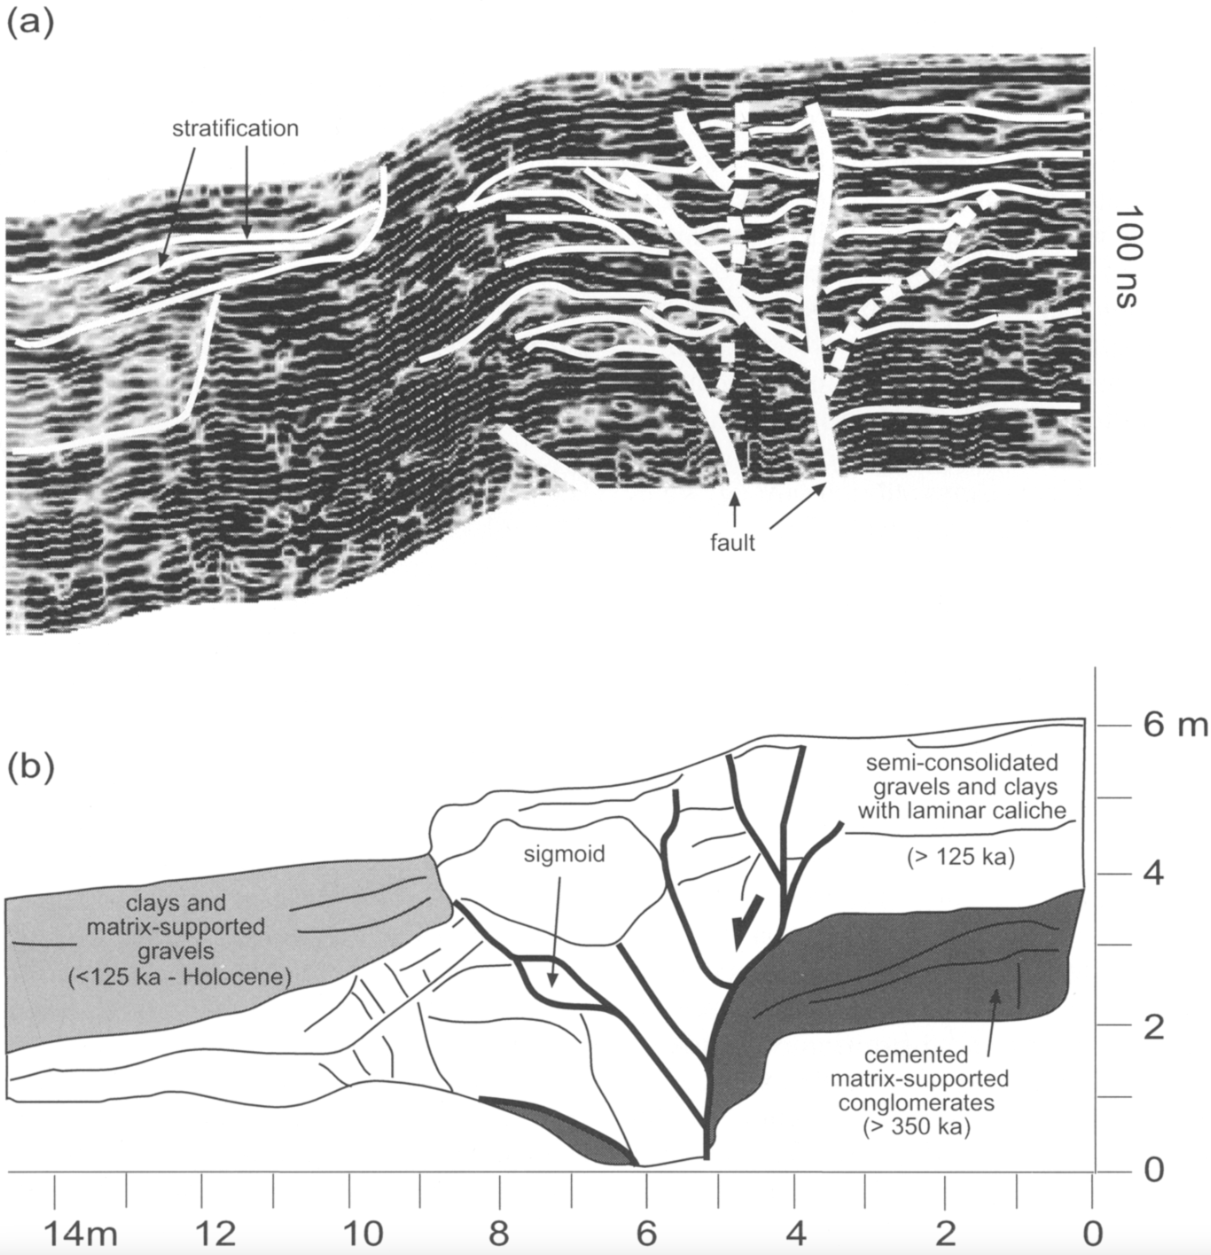
\includegraphics[width=0.9\linewidth]{Figures/0.2GPR/reiss2003_normal-faults_1.png}
    \caption[Active normal faults and associated sediments (1).]{Active normal faults and associated sediments (1).\textbf{Keywords: } Sigmoid, faulting, discontinuous, parallel, stratification, medium amplitude \citep{Reiss2003}.}
    \label{fig:Reiss2003-1}
\end{figure}

\begin{figure}[h!]
    \centering
    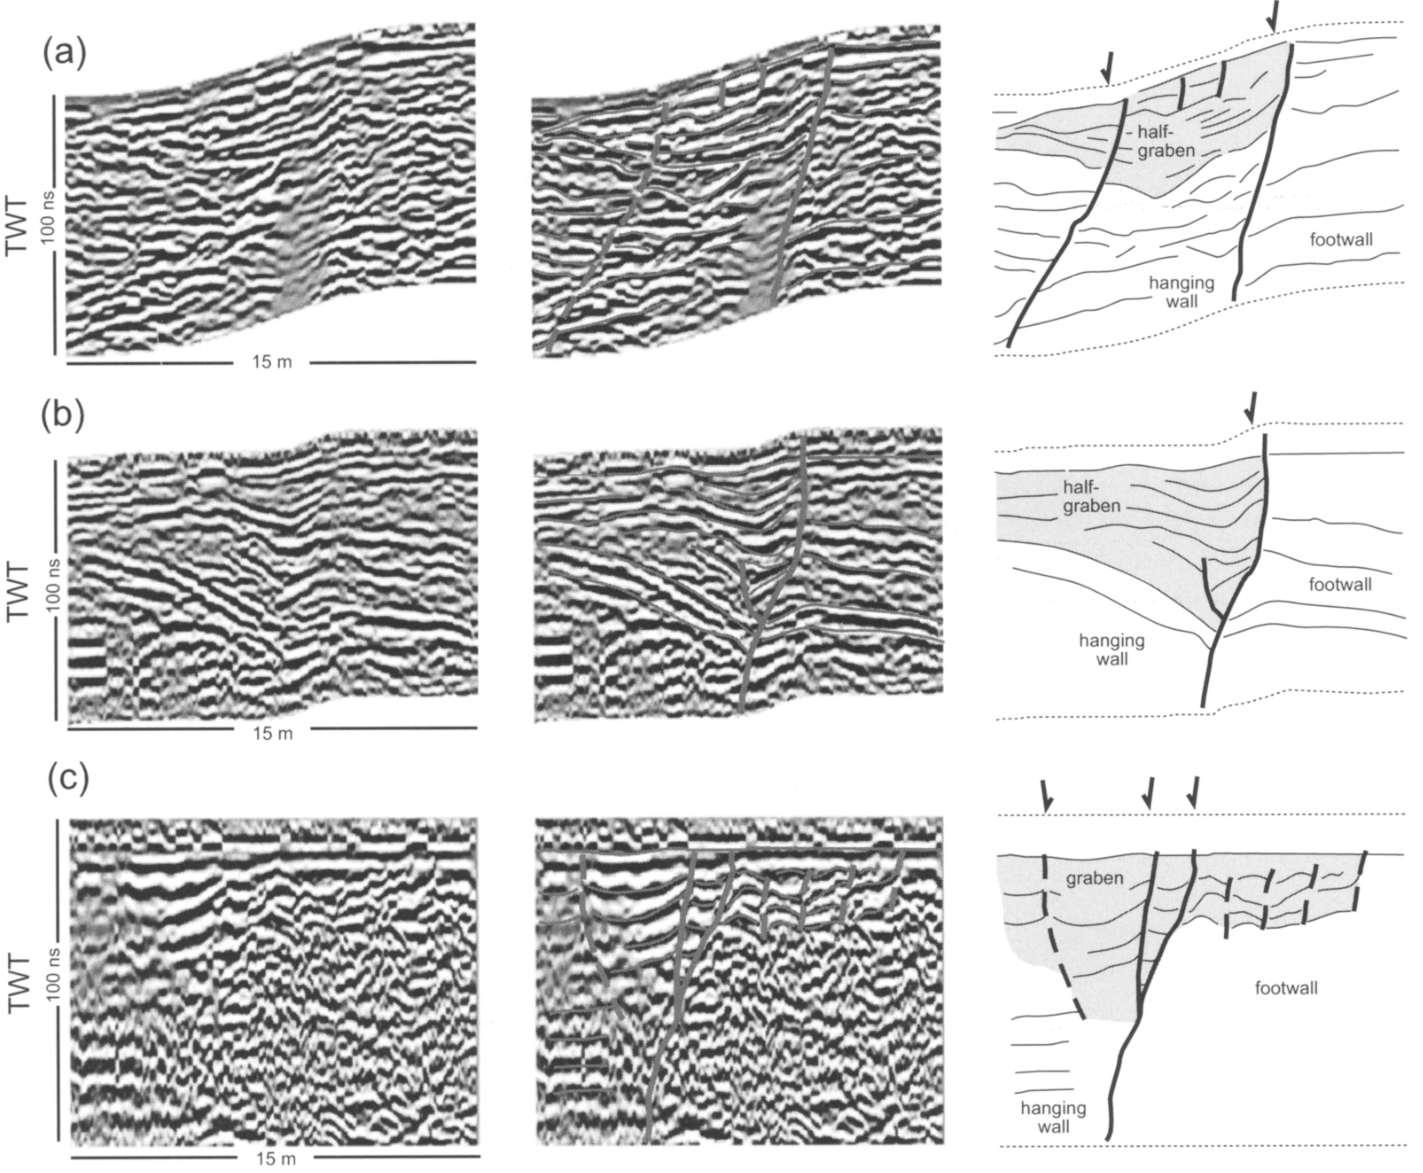
\includegraphics[width=0.9\linewidth]{Figures/0.2GPR/reiss2003_normal-faults_2.png}
    \caption[Active normal faults and associated sediments (2).]{Active normal faults and associated sediments (2). \textbf{Keywords: } Dipping, parallel, crossing reflectors, discontinuous, high amplitude \citep{Reiss2003}.}
    \label{fig:Reiss2003-2}
\end{figure}